\chapter{Design}
Systemet er opdelt i tre dele, klienten, serveren og compileren. Alle af dem er skrevet i Dart\footnote{Dart er et ny sprog fra Google til at afløse Javascript},
Databasen var bestemt på forhånd til at være en Postgres server og skemaet lå også klart.

\section{Database}
\begin{figure}[ht!]
\centering
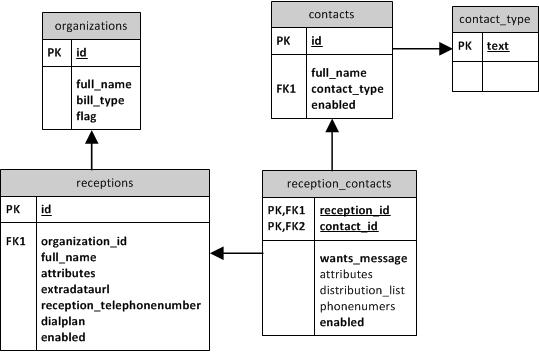
\includegraphics[scale=0.7]{images/ER_Basic.png}
\caption{Udsnit af database skemaet. PK er Primary key. FK er Foreign Key. Tekst i fed skrift er obligatoriske felter}
\label{fig:erbasic}
\end{figure}
Datamodellen er lavet så først har man organizationer, som beskeriver hvem der skal sendes regninger ud til og hvordan de ønsker dem, samt at den samler flere receptioner. En reception er den kontekst som der bliver ringet ind til. Så i større virksomheder vil der være flere som f.eks. afdelinger eller forskellige butikker rundt omkring i landet og i små virksomheder vil der typisk kun være en reception. En reception indeholder information om blandt andet hvordan de ønsker håndtering af sælgere, hvad deres CVR numre er og helt lavt praktisk hvad addressen er eller hvad deres åbningstider er. En virksomhed er ikke noget uden deres medarbejder, så til dem er der kontakter som beskriver personen ved deres navn. Det er først i forbindelse med en reception at en kontaktperson har det meste af sin information, som hvad deres telefonnumre og email er, samt information omkring hvad de har af ansvar og hvem deres backup personer er, og den information gemmes i ReceptionContacts tabllen.
Databasen har en mere flere tabeller end beskrevet her og diagrammet for det fulde database skema kan findes i bilaget.

\section{Server}
Serveren er bygget op efter MVC arkitekturen, da det passer godt til hvordan en websevrer kan sættes sammen og er godt til at holde de forskellige dele adskildt. Derved har den en rækker controller som står for at håndtere forespørgelserne. De fleste af dem, omhandler blot at hente data ud fra databasen og sende dem ud til brugere. En sådan controller går altså til databasen, får tilbage dataen i typer fra modellen som bliver transformeret om af et view, så dataen kan blive sendt ud til klienten.
Controllerne er i højgrad opdelt efter hvordan datamodellen på databasen er bygget op. 

Dialplans. Compiler til XML som freeswitch forstår i stedet for at have en service som den kalder ud til for at finde ud af hvad den skal nu. Stabilitet, 

%\pagebreak
\section{Brugerfladen}
Brugerfladen er blevet skitseret i samarbejde med Adaheads K/S, så den falder ind sammen med resten af systemet.
Den er bygget op, så i venstre side har man en menu hvor man kan vælge imellem organisationer, receptioner, kontakterpersoner og dialplan. Alle 4 vinduer er bygget op omkring 3 søjler for at holde det konsistent.

\subsection{Organisationer}
\begin{figure}[ht!]
\centering
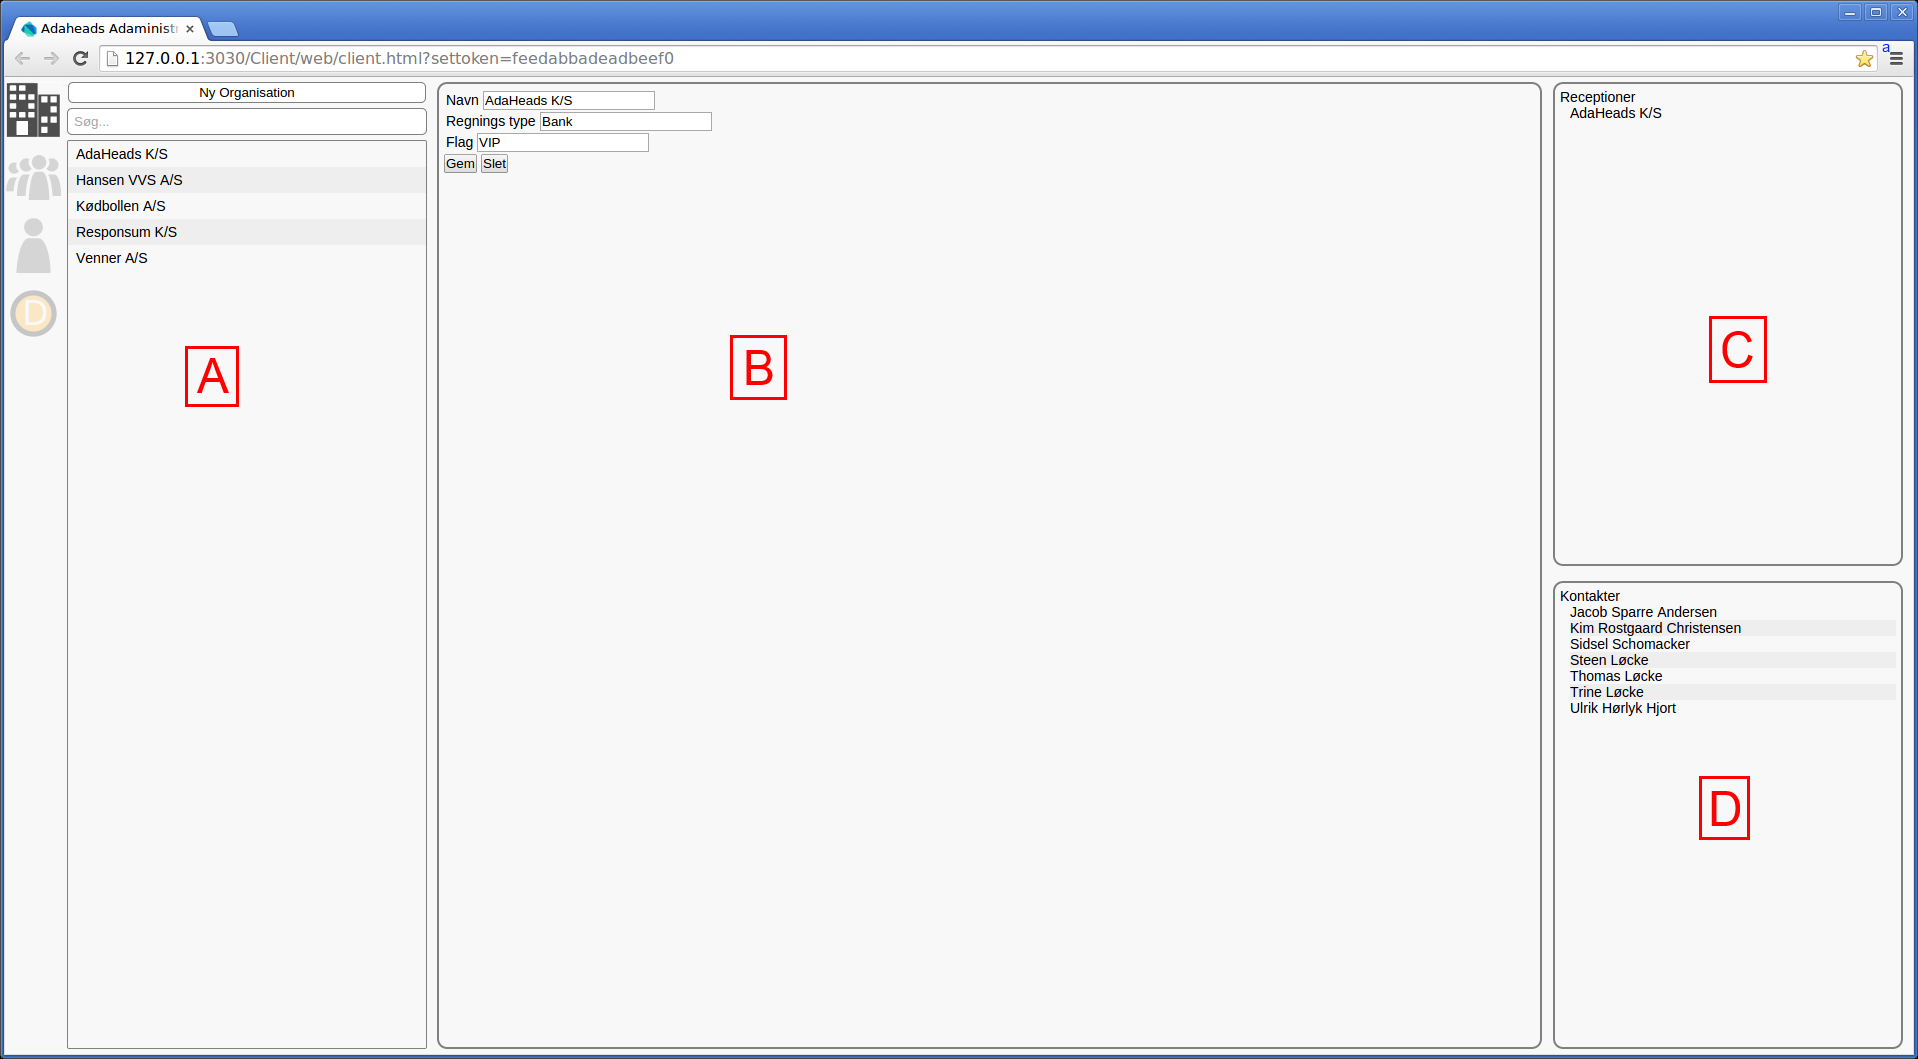
\includegraphics[width=\textwidth]{images/screen_org.png}
\caption{Organisation redigering}
\label{fig:screenorg}
\end{figure}
På organisations vinduet kan man ude i venstre side se en liste af alle organisationer som er tastet ind, og i toppen af den kan man enten skrive i søgefelter som filetere listen neden under eller trykke for at oprette en ny. I midten kan man indtaste information omkring den pågældende organisation. I den højre søjle er der to lister. Den ene med receptioner og den anden med kontaktpersoner der til hører den valgte organisation.

\subsection{Receptioner}
\begin{figure}[ht!]
\centering
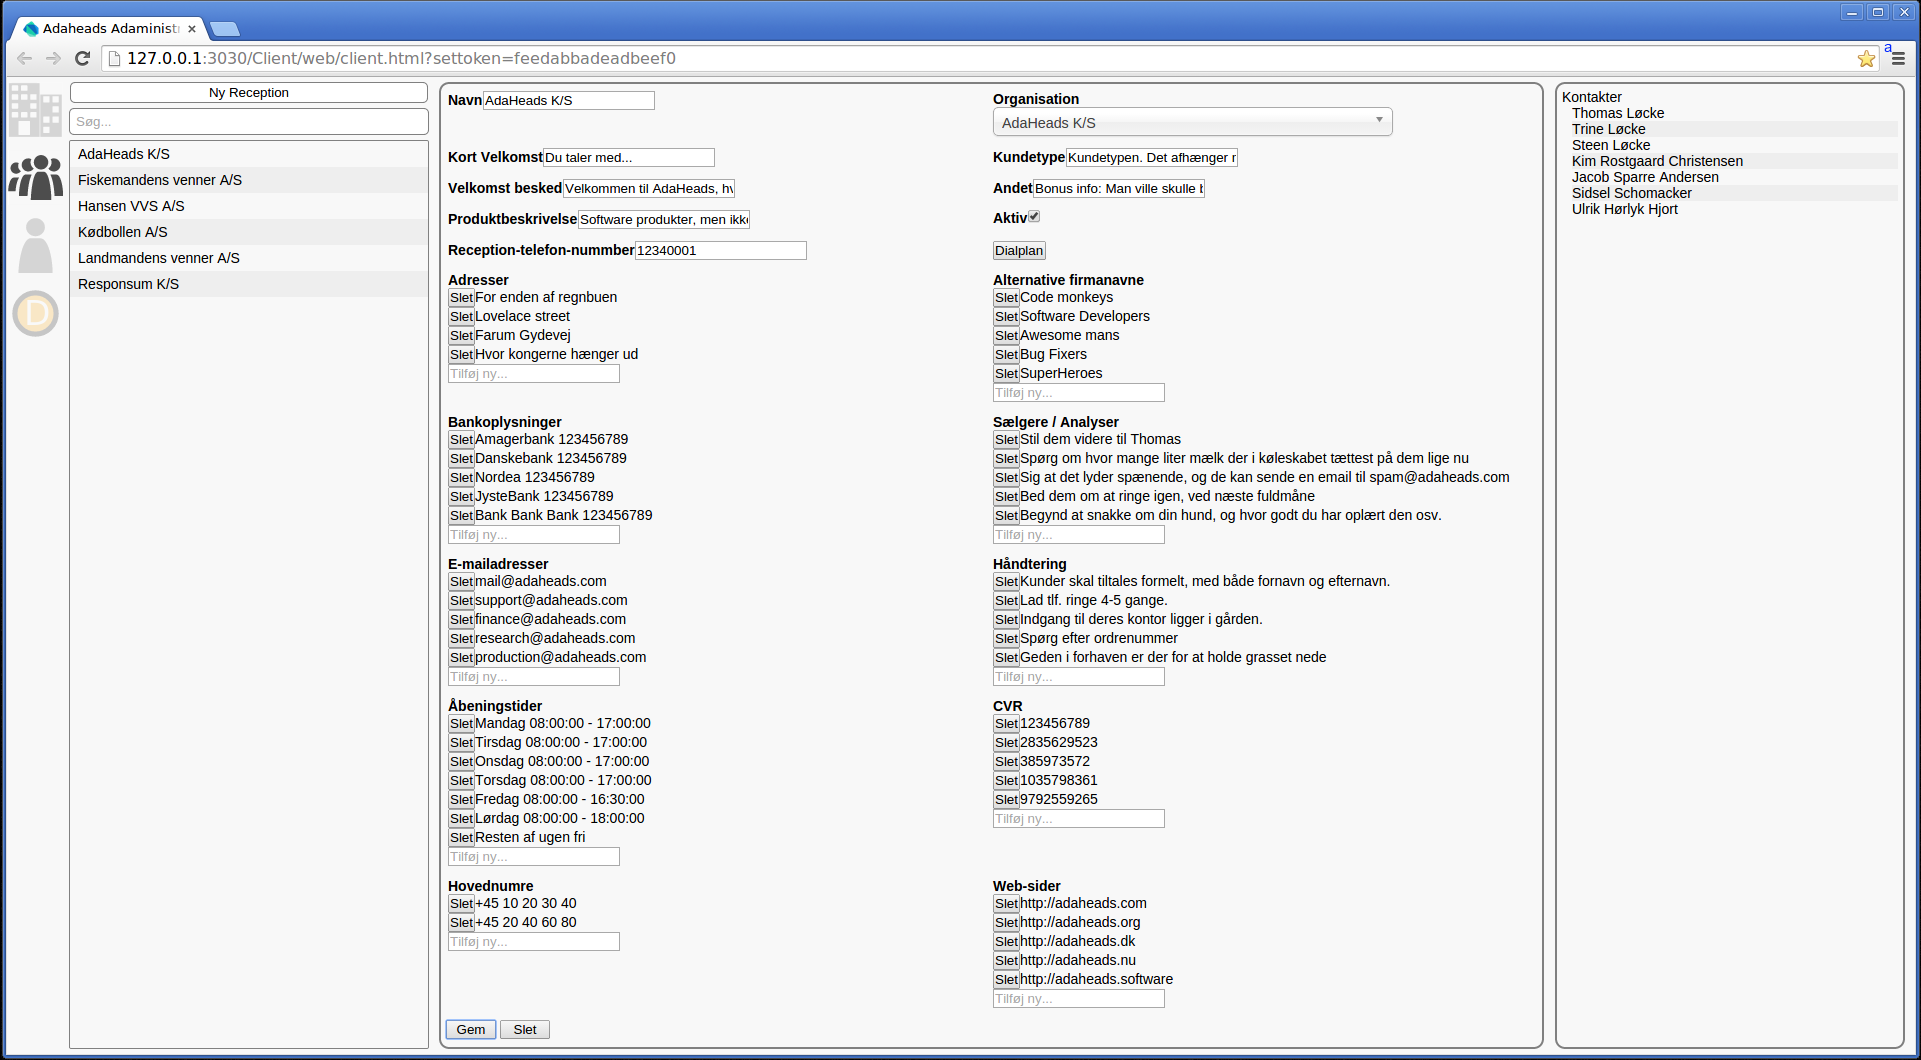
\includegraphics[width=\textwidth]{images/screen_rec.png}
\caption{Reception redigering}
\label{fig:screenrec}
\end{figure}
Receptions vinduet er lavet i meget samme stil som organisationvinduet. Det har også startede fra toppen i venstre siden, en søjle hvor der oprettes nye receptioner, et søgefelt for listen neden for, der indeholder alle receptioner. I midten er søjlen med informationen omkring en reception, og til højre er der en søjle med alle kontaktpersoner for receptionen.

\subsection{Kontaktpersoner}
\begin{figure}[ht!]
\centering
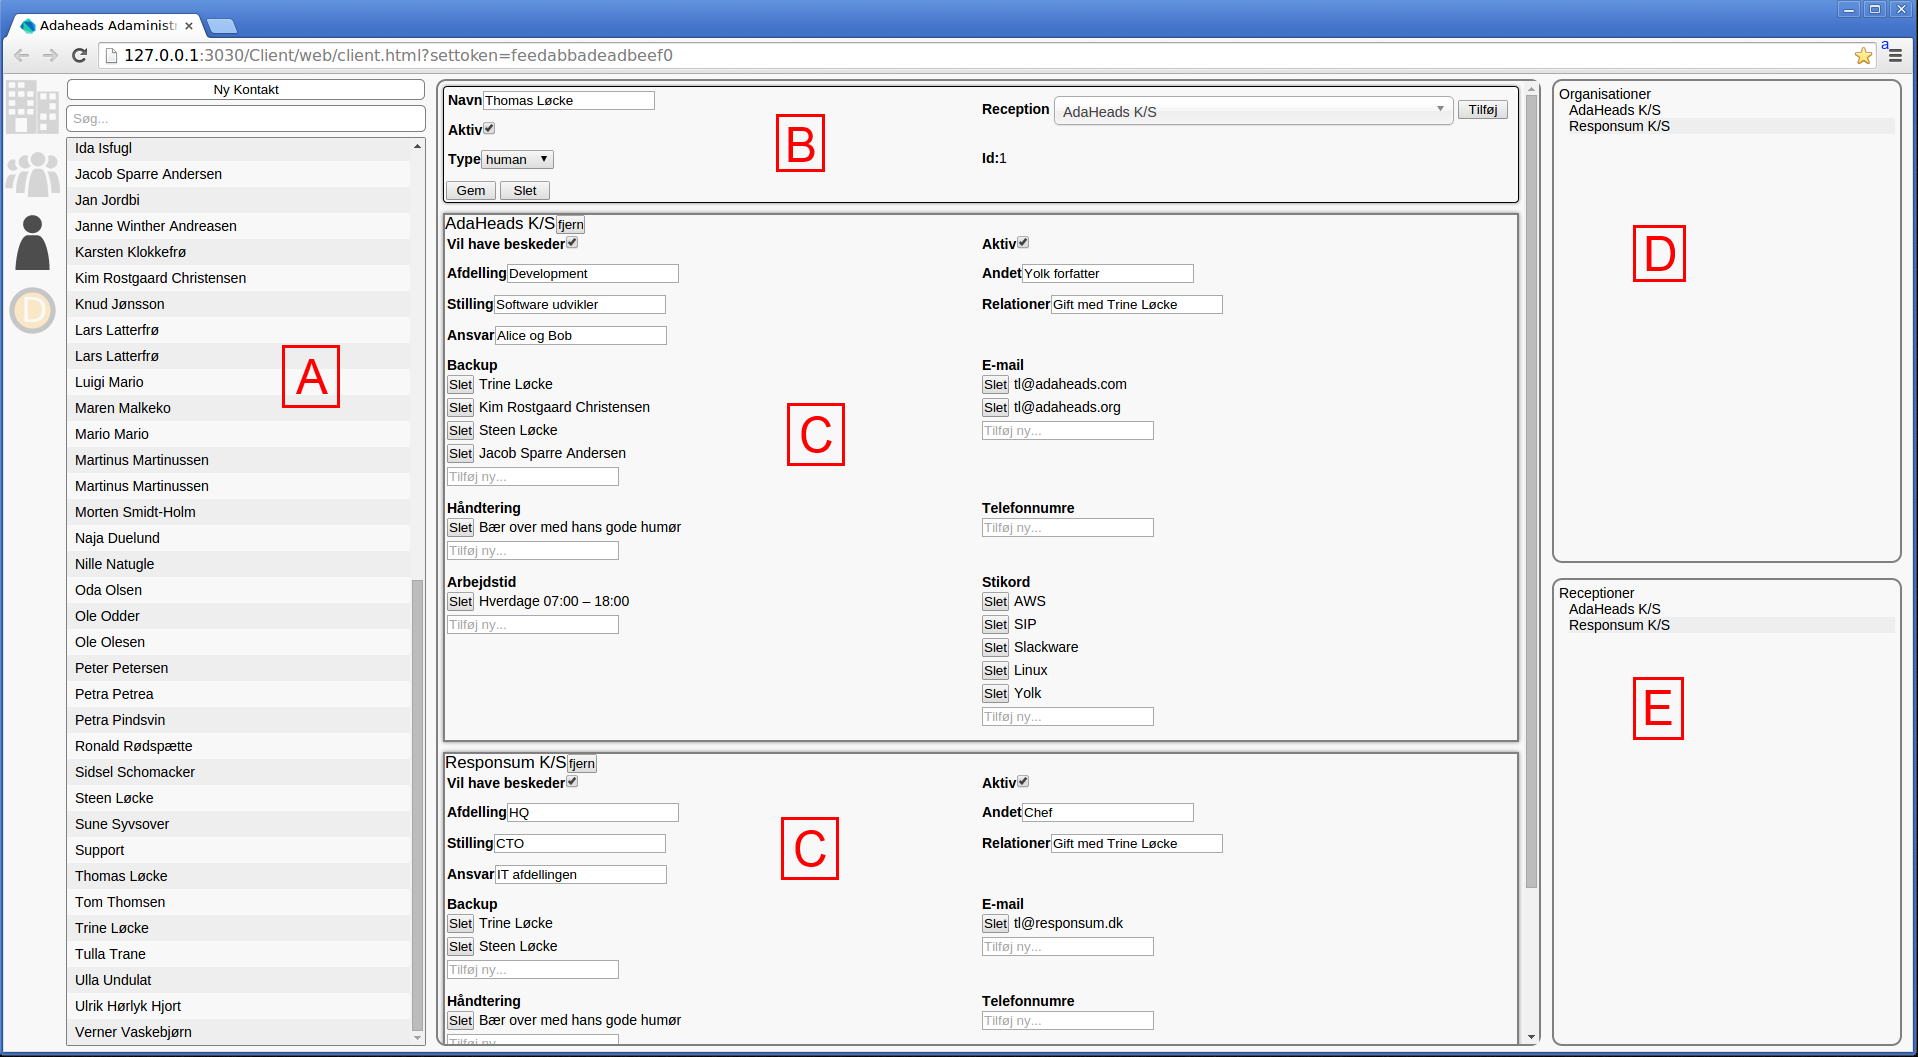
\includegraphics[width=\textwidth]{images/screen_con.png}
\caption{Kontakter redigering}
\label{fig:screencon}
\end{figure}
I vinduet for kontaktpersoner er der lige som i de forrige to, opret knap, søgefelt og i vinduet her er det en så en liste over kontaktpersoner. I toppen af søjlen i midten er der information omkring en kontaktperson, hvor der er mulighed for at tilknytte en kontakt til en reception. Har en kontaktperson en tilknytning til en reception, så optræder der en boks med alle information tilknyttet til den relation. I højre side er der to lister henholdvis hvilke organisationer og receptioner som kontakten optræder i.

\subsection{Dialplan}
\begin{figure}[ht!]
\centering
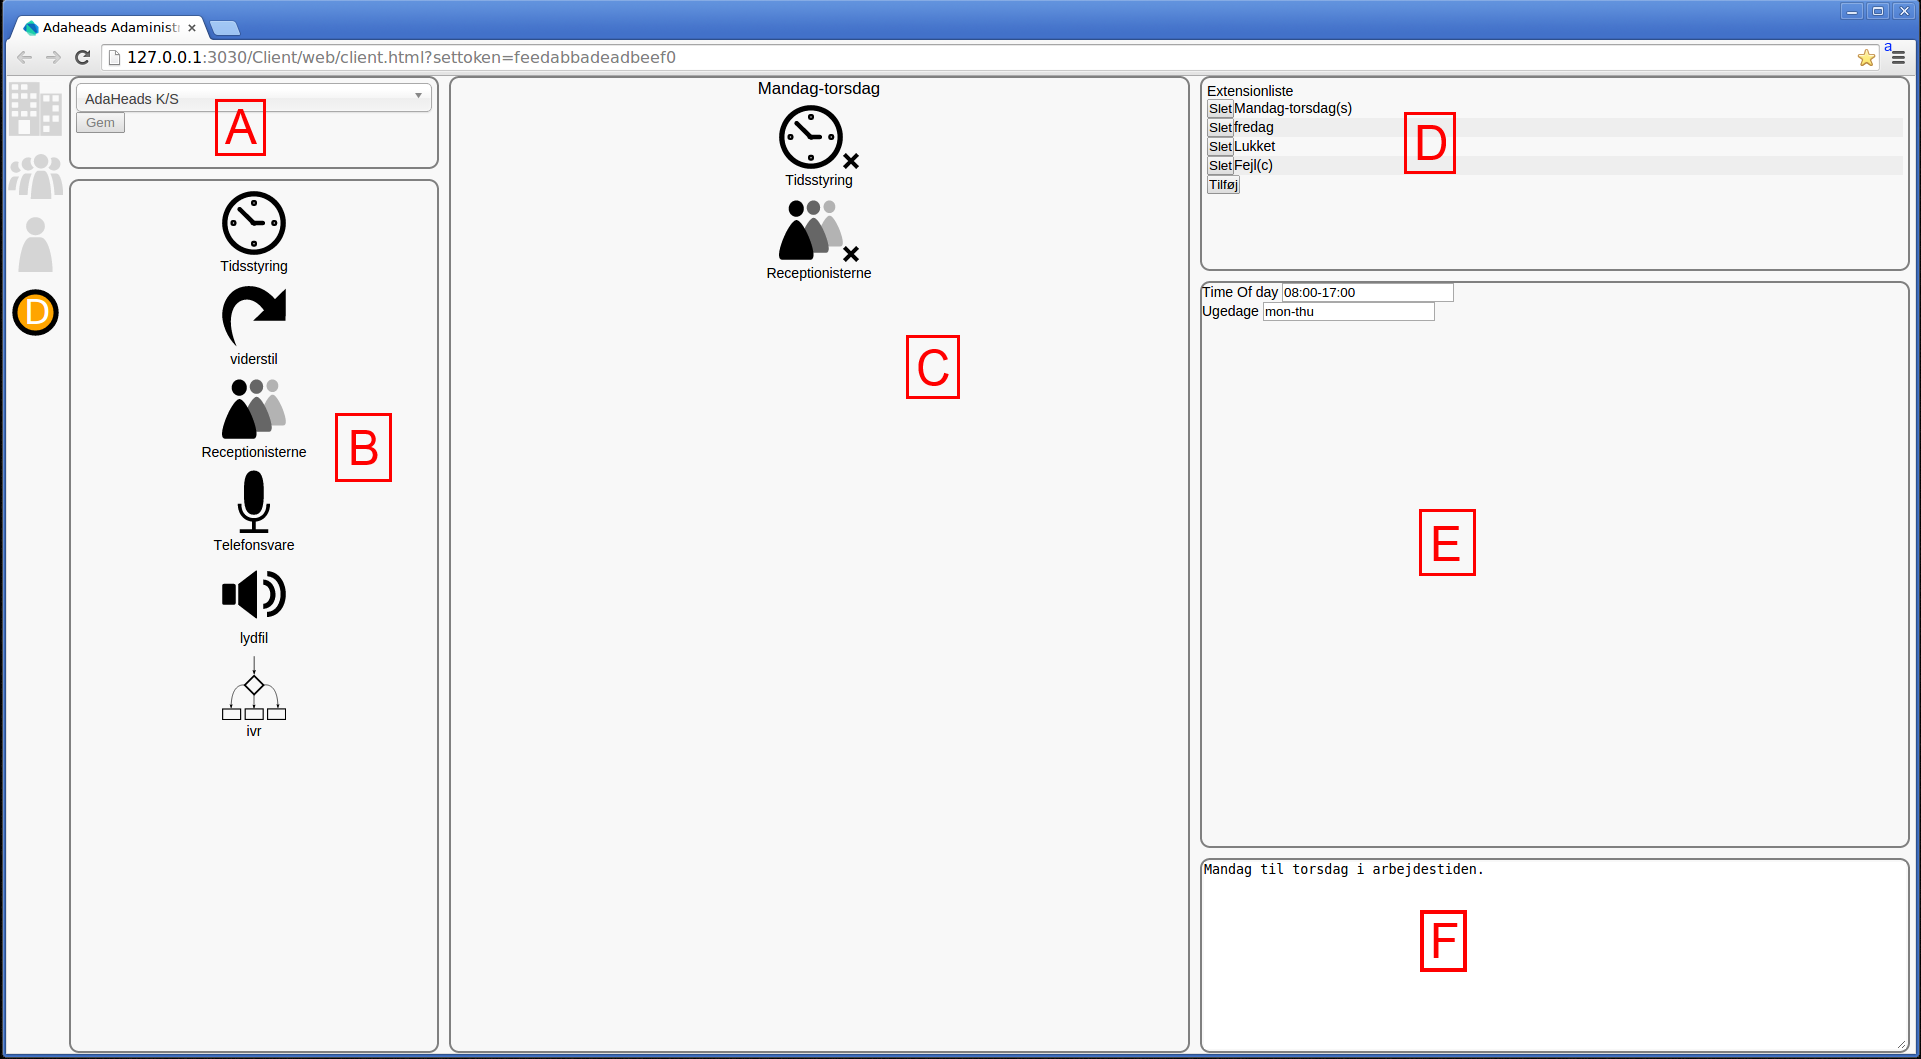
\includegraphics[width=\textwidth]{images/screen_dialplan.png}
\caption{Dialplan redigering}
\label{fig:screendialplan}
\end{figure}
Til at lave dialplans er der også lavet et vindue til det. Det er også bygget op med af tre søjler. I den første søjle kan man i toppen vælge en reception, og når man har lavet ændringer så kan man trykke på gem knappen lige uden, som sender dialplan tilbage til serveren hvor den bliver gemt. Under den kasse kan man vælge imellem de forskellige handlinger og betingelser der skal ske i en extension. Når man så trykker på en af dem bliver den indsat i dialplanen og vist i midten, hvor man kan se forløbet af opkaldet og trykker man så på dem der, kan man få vist dens indstillinger, der kommer frem ude i den højre søjle, hvor det også er muligt at se en liste over extensions for den givende dialplan.

%\begin{figure}[ht!]
%\centering
%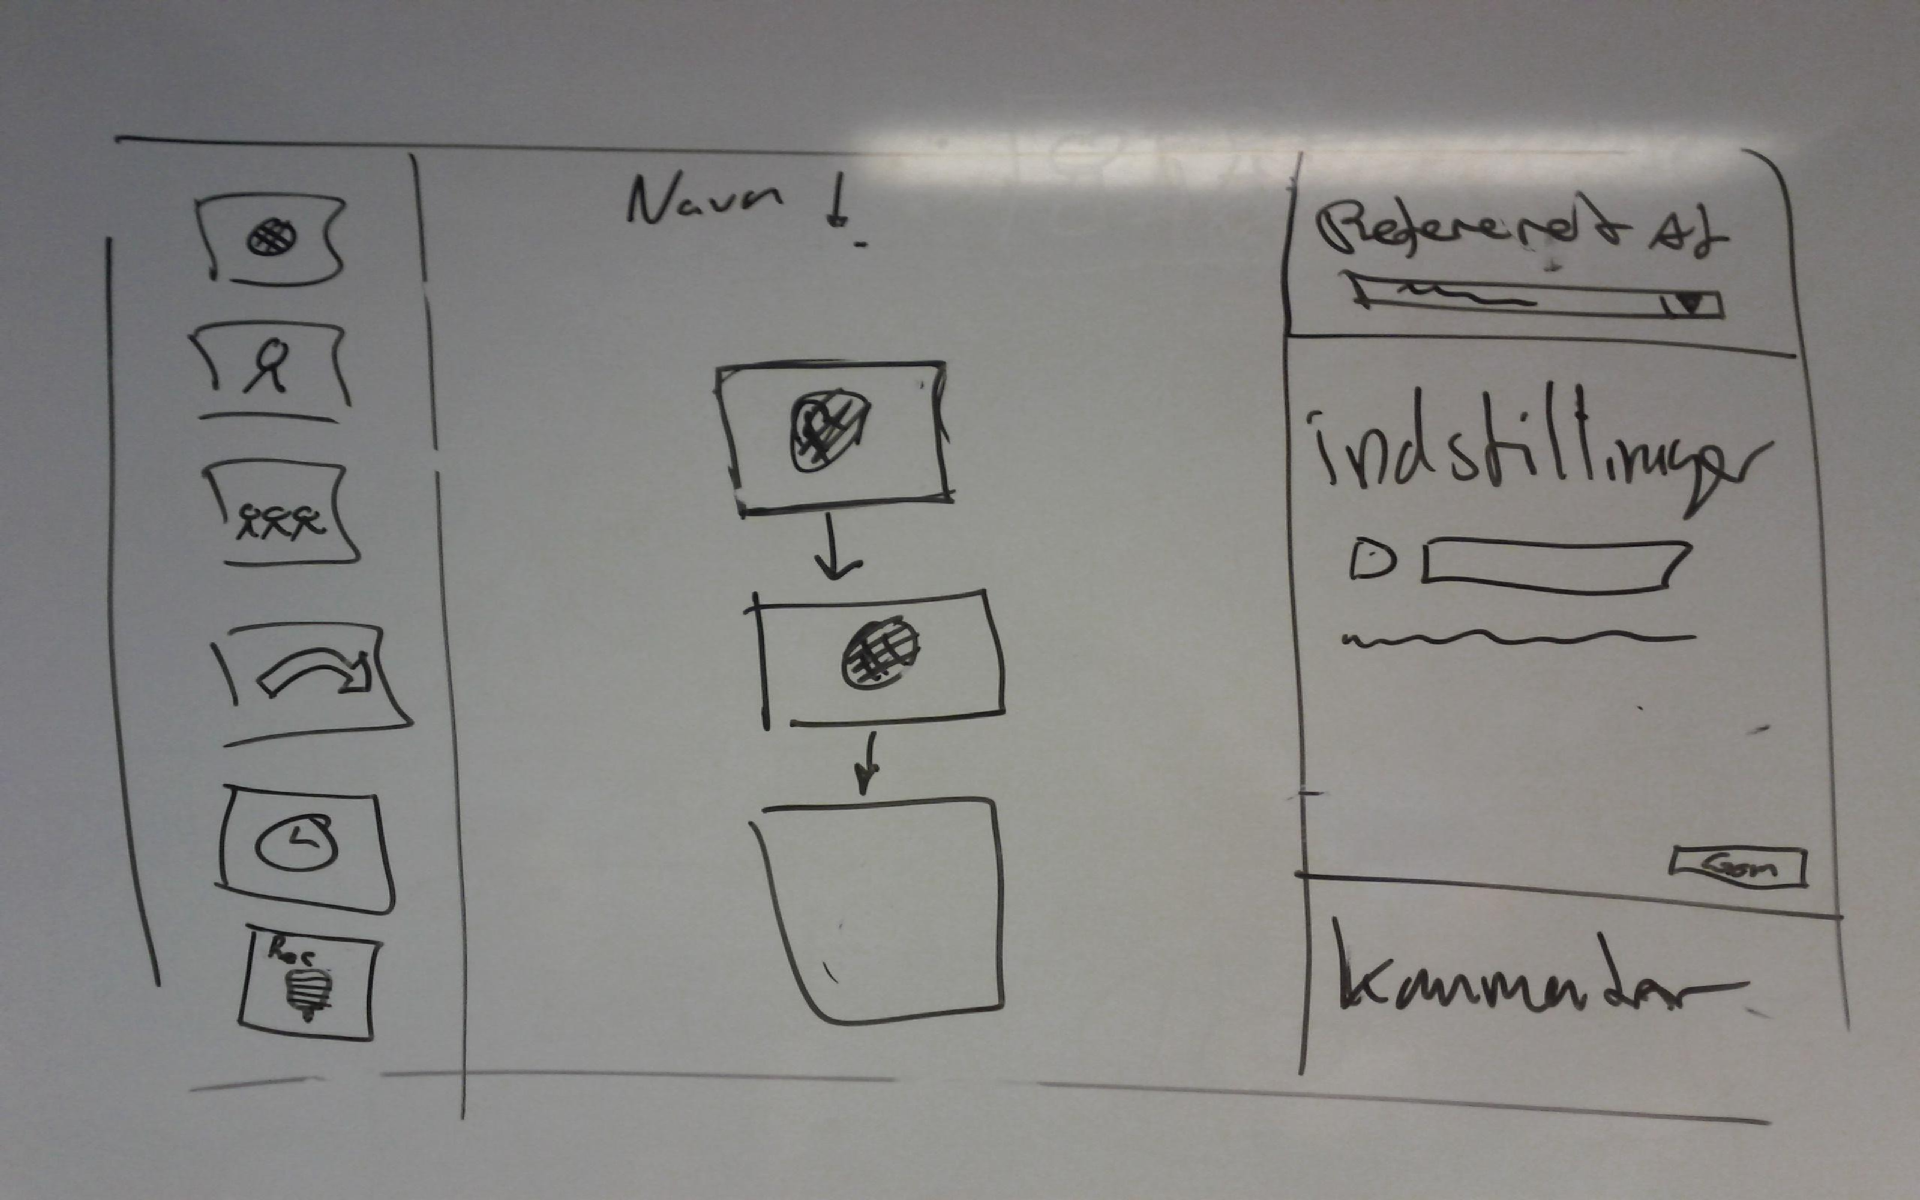
\includegraphics[scale=0.21]{images/dialplansketch.png}
%\caption{En skitse over hvordan dialplaner laves.}
%\label{fig:dialplansketch}
%\end{figure}

%\pagebreak
%\section{Program arkitektur}
%Klasse Diagram og sekvensDiagram???
%Klasse:
%    Controller, Database, views, model
%    
%sekvens:
%    Request -> HttpServer -> Router -> AUTH <- Router -> Contrller -> Database -> View -> ....(The End)
%
%
%Dette er til arkitekturen...

\section{Dialplans}
Freeswitch er bygget op af en kerne der i sig selv ikke kan bruges som PBX, men med de moduler som følger med kan den bruges til at forbinde IP telefoner eller andre PBX'er, transkode lyd, afspille IVR menuer eller hvad man selv kan finde på at skrive i et modul.
Når der kommer et opkald ind i telefonanlægget, skal det vide hvordan det skal håndtere opkaldet. I en PBX kalder man det en dialplan.  
I Freeswitch kan man skrive sin dialplan i en række af programmeringssprog, men som standart bliver der brugt et modul kaldet mod\_dialplan\_xml og som navnet fortæller så bruger den XML til at beskriver dialplanen. Der er også den mulighed at lave det, de kalder en indbound socket som fungere ved at man forbinder til deres socket, og der hvor den før hen havde gået ned og læst hvilke applicationer der skulle afvikles, så spørger Freeswitch i stedet for på denne forbindelse i stedet for. Adaheads K/S valgte at bruge mod\_dialplan\_xml og derved skrive deres dialplan i XML. Det giver den fordel at mod\_dialplan\_xml er et gennemprøvet produkt og når der skal laves ændringer til en dialplan så kan man ændre i filerne og bede Freeswitch om at genindlæs dens dialplans, hvilket ikke giver nogen nede tid. Den mere dynamiske tilgang med en socket er mere fleksibelt, men den statisk udgave ser ud til at kunne det Adaheads kræver af det.

\section{Mod\_Dialplan\_XML}
En dialplan er bygget op af en række lag.
\begin{figure}[ht!]
\centering
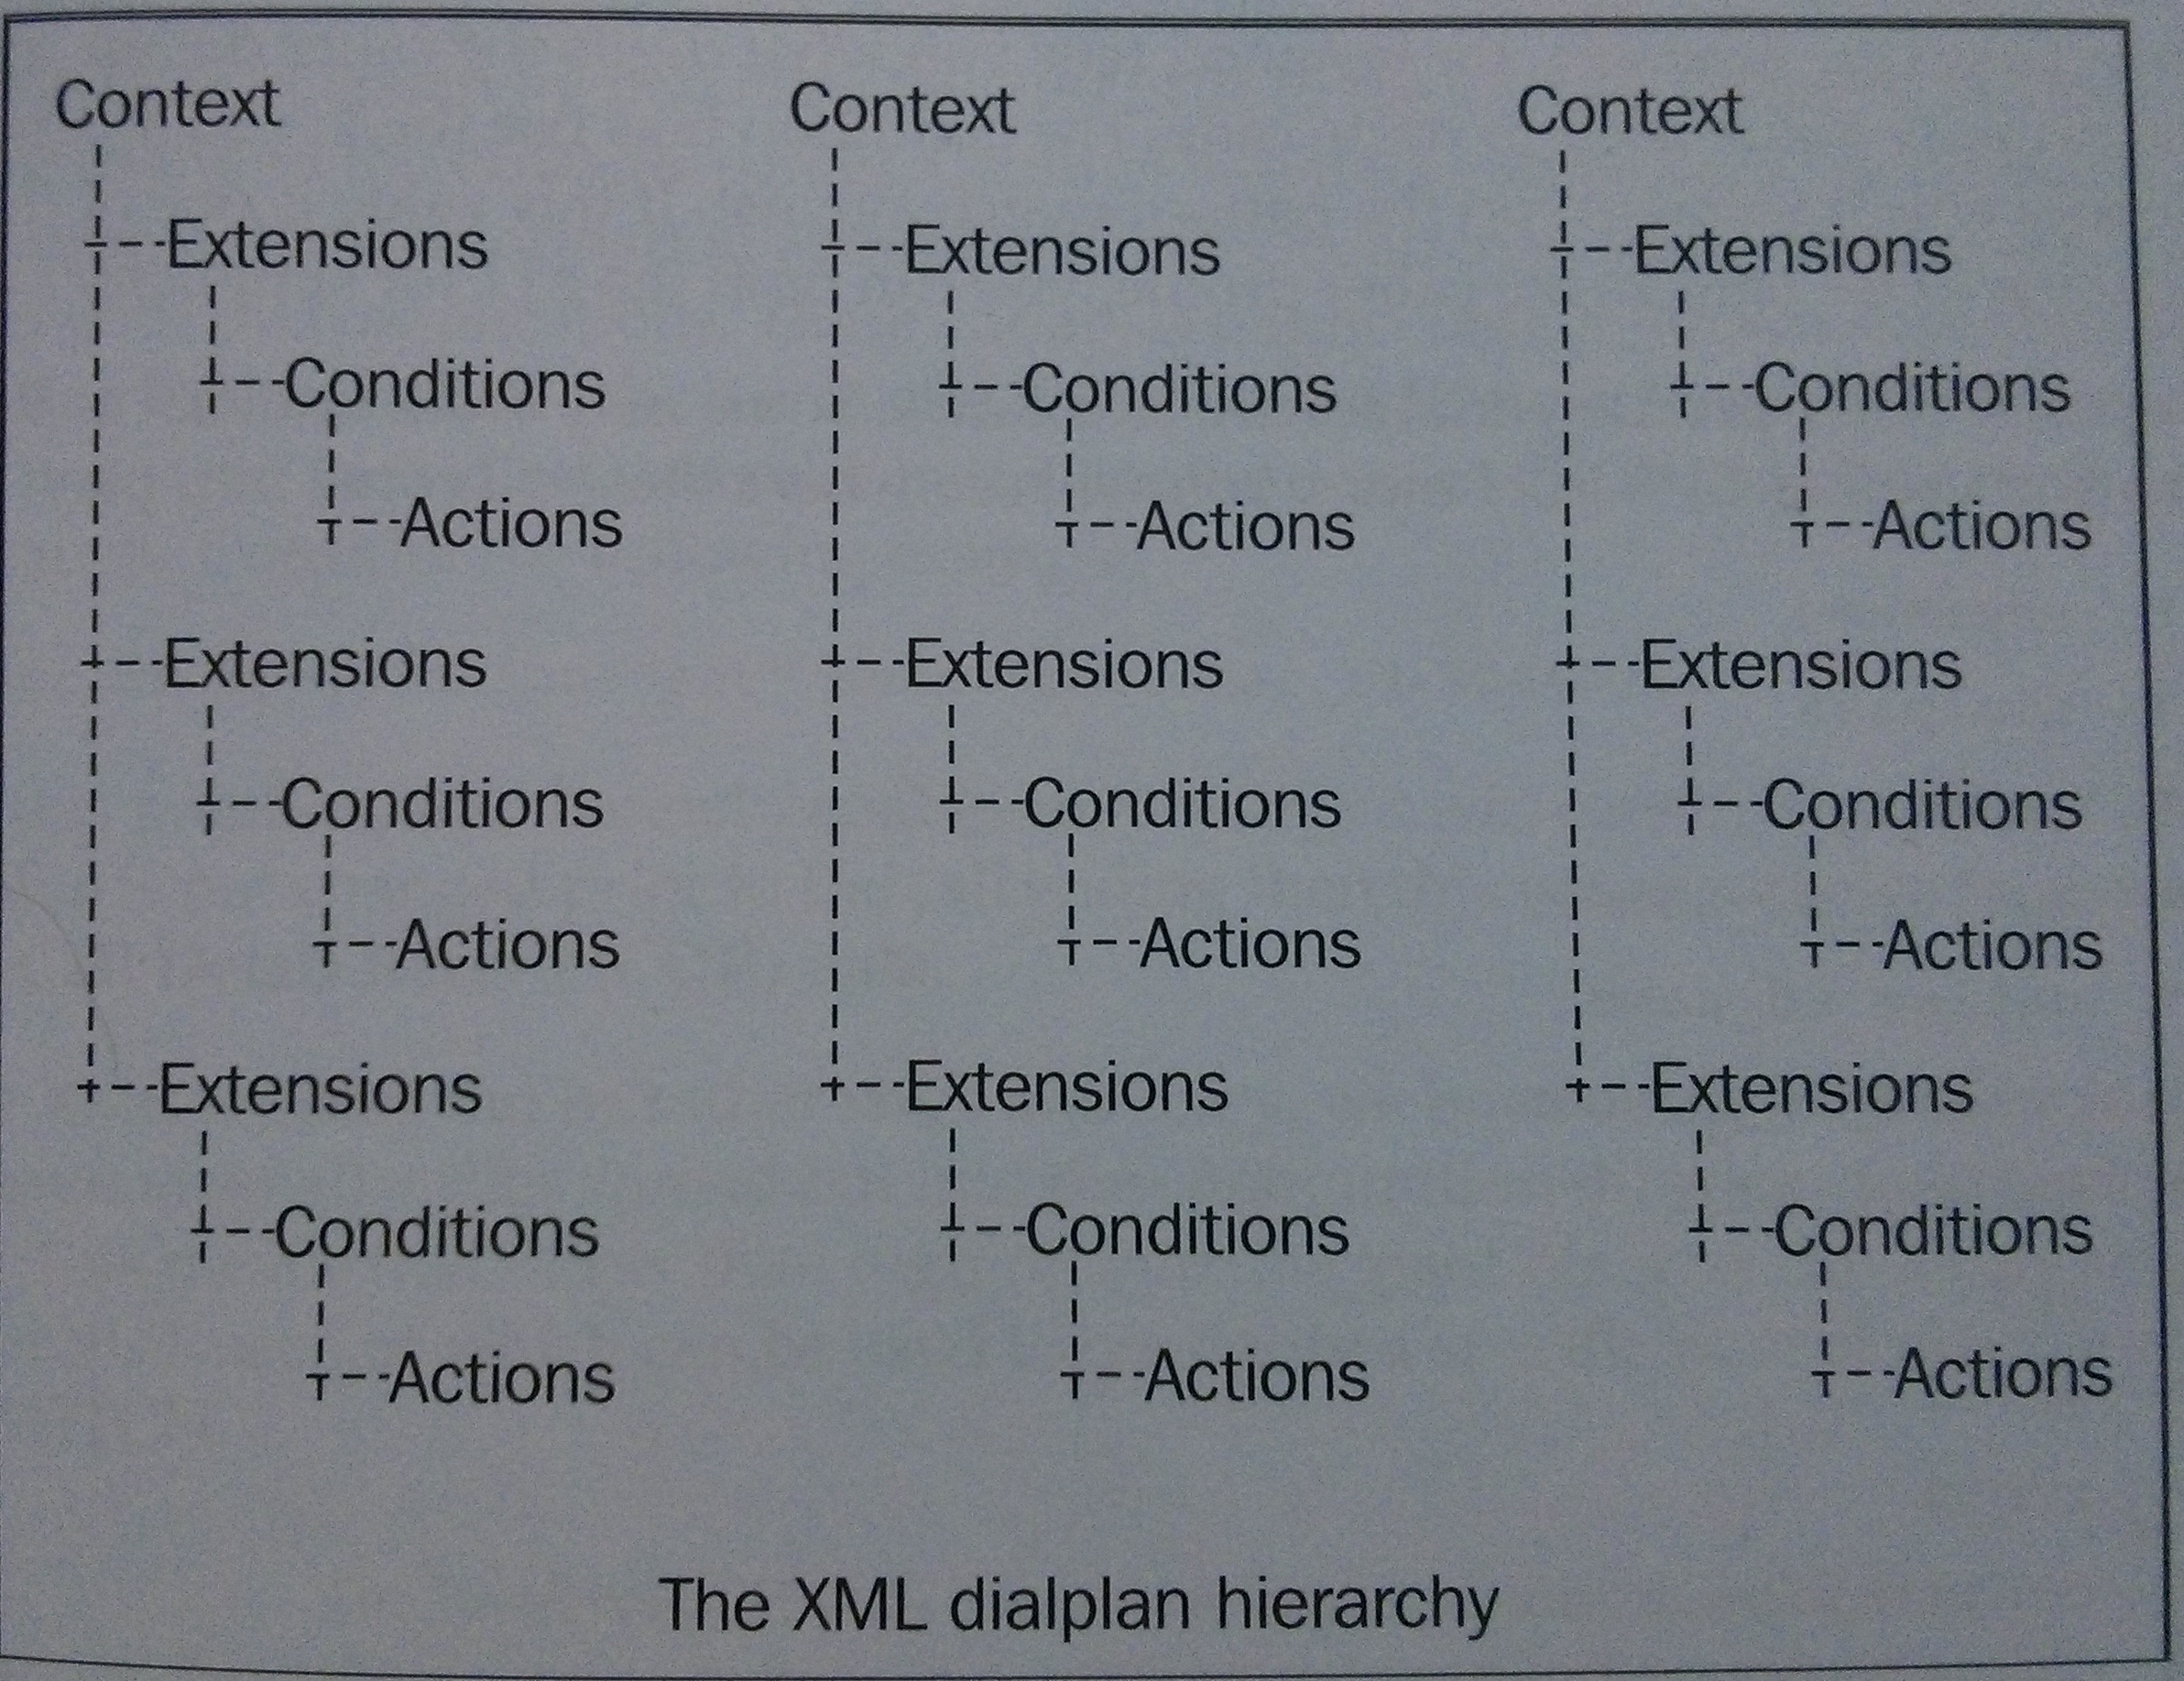
\includegraphics[scale=0.14]{images/dialplanstructure.jpg}
\caption{Strukturen for en XML dialplan\citep{freeswitch12}}
\label{fig:xmldialplan}
\end{figure}
Det først lag er Context. En Context er specificeret ved et unikt navn, den kan bestå af flere Extensions og en Dialplan kan have flere dialplans. Når man registrer en telefon, eller en PBX så konfigureres en context der ringes ind i. Det har den fordel af man kontrollere hvilke extension som kan ringes ind til fra hver telefonerne og for hver af PBX.
Det næste lag er for extensions. En Extension er en gruppering af conditions.
Conditions er som navnet beskriver, de betingelser der skal opfyldes. Hvis alle conditions i en extension er opfyldt bliver alle actions udført, men hvis der er en condition som ikke er, bliver den conditions anti-action udført. En condition har indbygget funktionalitet til at tjekke på en masse ting omkring tid. F.eks. om det er mandag, eller om klokken er mellem 08:00 og 09:00, hvilet år det er osv. Men udover det kan man kalde andre applikationer og ved hjælp af Perls Regular Expression der bruges til at tjekke svaret, udbygge det til at tjekke hver som helst. 
Actions og anti-actions er det samme, det eneste der skiller dem ad, er i hvilke omstændighed de bliver udført. Actions er bygget op helt simplet, ved at man specificere et applikationsnavn og dens parameter.

\pagebreak
\section{SystemOversigt}
Det samlet system består af flere maskiner. Den første har Freeswitch og står dermed for at snakke sammen med andre telefonanlæg ude i verden, samt de telefoner som receptionisterne bruger. På den samme maskine er generatoren der har adgang til databasen, til når dialplans, IVR menuer eller andre dele af den skal konfigureres. Det næste led i kæden af maskiner er der hvor Adaheads K/S CallFlow-Control program kører, der opdager nye opkald og sørger for at fortælle klienten om det foruden en masse andre ting også. Det er også her webserveren til det administrative kommer til at køre, selv om det ikke er nødvendigt at de er på samme maskine. Til sidst er der klienten der blot skal have en moderne browser for så at kunne kommunikere med webserveren.

\begin{figure}[ht!]
\centering
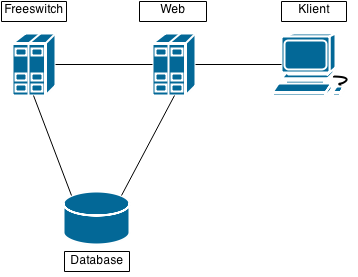
\includegraphics[scale=0.8]{images/systemdiagram.png}
\caption{Diagram over systemet.}
\label{fig:systemdiagram}
\end{figure}


\section{REST}
Serveren er lavet efter principperne i REST.
REST (\textbf{RE}presentational \textbf{S}tate \textbf{T}ransfer) er en web arkitektur der blev opfundet af Roy Fielding i hans ph.d.-afhandling. I den beskriver han at denne arkitektur bygger oven på HTTP og at serveren som klienten snakker med skal være tilstandsløs. Det har en række fordele. Når transportlaget ikke skal holde nogen tilstand, så kan det spare på de fysiske ressourcer og på den måde opnå højere skalerbarhed. Det betyder også at man kan sende forspørgelser parralellet og at der kan kører flere instanser af serveren, og klienten behøver ikke vide hvilken en der snakker med.
REST er bygget op så man benytter sig at HTTPs method header variable. Så ønsker man f.eks. at fjerne et element så spørger efter den pågældende ressource med method sat til DELETE.

















